\section{Algorithms}
\graphicspath{ {Images/} }

\subsection{Reinforcement Learning (RL)}\label{RL}
We use a reinforcement learning approach to implement three types of agents. Reinforcement learning is a type of machine learning where behavior is learned through trial-and-error interactions with the dynamic environment. Agents, or learners, determine which action to take in order to maximize  its reward. Most of the time the action with the highest expected reward is taken, which is called exploitation. Exploration is taking a new action that has not previously been taken in the same state to learn that action's utility in the current state. The exploration-exploitation trade-off is among the biggest challenge in RL. Figure-\ref{fig:res} illustrates this learning process.

%Reinforcement Learning is a form of Unsupervised Learning where agents, or learners, do not have any prior data to learn from. The learner is not told which actions to perform, but instead must discover which actions yield the highest reward by evaluating the state after performing an action. Each action is associated with a reward and based on the rewards obtained, the learner learns the best future actions to take.

 %There are two main players in any reinforcement learning
 %\begin{enumerate}
 %\item {\bf{Agent: }} learner or the decision maker~\cite{Busoniu08CompSurvey}
 %\item {\bf{Environment: }}  Things with which the agent interacts.
 %\end{enumerate}
 
 
 
 \begin{figure}[htb]

\begin{minipage}[b]{1.0\linewidth}
  \centering
  \centerline{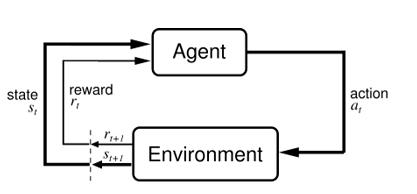
\includegraphics[width=6.5cm]{RL}}
%  \vspace{2.0cm}
  
\end{minipage}
\caption{ Agent-Environment interaction in Reinforcement Learning~\cite{Sutton98reinforcementlearning}}
\label{fig:res}
%
\end{figure}

In our case, agent is the unit of a team and state is the map of all visible units and empty positions. During each turn, the agent calculates all the possible actions in its current state and assigns an initial value to each state. This mapping is called the agent's policy. Units pick actions based on the exploration-exploitation techniques of the underlying MARL algorithms controlling each team.

A unit receives a positive reward when it kills an enemy unit and a negative reward when it is killed or kills an ally. Reward values range from [-2,1], with the highest reward for killing an enemy, 1, and the lowest rewards for killing an ally or getting killed, -1 and -2 respectively. Rewards are also given for proximity to enemy units, 0.5, and ally units, 0.25.

\subsection{\MARL\ (MARL)}\label{MARL}
We use three variants of MARL to compare the effects of message-sharing between units. In MARL, multiple agents apply RL in a shared environment and collaboratively learn a single objective. Here the policy function depends not only on the environment but also on the policies of other agents. Figure-\ref{fig:res2} explains the model of MARL.
 
\begin{figure}[htb]

\begin{minipage}[b]{1.0\linewidth}
  \centering
  \centerline{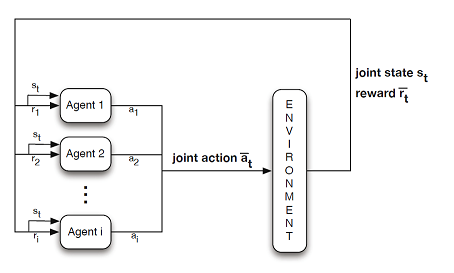
\includegraphics[width=8.5cm]{MARL}}
%  \vspace{2.0cm}
  
\end{minipage}
\caption{ Multiple agents acting in the same environment~\cite{Nowe12GameTheoryMultiAgentReinforcement}}
\label{fig:res2}
%
\end{figure}

 At each step, a joint action from all agents acts on the environment. A joint action is a vector of actions, one action per agent. The joint action acting on the environment changes the shared state and produces a reward for each agent based on the action the agent took.
 
 In our game, each team has a joint action separate from the opposing team, so at each step, one of the two teams composed of multiple agents will perform a joint action on the environment. The state will change for both teams, but the rewards for each action will only go to the agents performing the action. Then the opposing team takes a step, and steps continue until the game ends.
 
 
 
\subsection{Q-Learning}\label{QL}
Q-Learning is a Reinforcement Learning technique in which each agent keeps an individual vector of values, Q-Values, corresponding to the possible action vector for each state, so that there is exactly one \qVal\ for each state-action pair. Initially, each \qVal\ is set to -2, but once the corresponding action is taken, the \qVal\ of that state-action pair is updated based on equation \ref{eqn:q_learn}.

\vspace{- 0.5 cm}

\begin{equation}\label{eqn:q_learn}
Q(t,a) = Q(t,a) + \alpha * [r(t,a) + \gamma V(t) - Q(t,a)]
\end{equation}


%\vspace{- 0.3  cm}

Here, $Q(t, a)$ is the \qVal\ for action $a$;  $\alpha$  is the learning rate; $r(t, a)$ is the reward function which returns the reward for taking the action $a$ in the given state $t$; $V(t')$ is the value function which returns the maximum \qVal\ for the next state multiplied by $\gamma$, a scaling factor, in order to back up the highest \qVal\ from the next state.



%In our game, the set of possible actions an agent can take are all the combinations of movement and attacking for a given state. A state is defined as the relative position of visible surrounding tiles and visible agents (friend or foe).

%Most of the time an action with the highest \qVal\ is picked. Sometimes agents choose to explore an action which has not been taken earlier. By exploring an action never taken, it is possible the action results in a state yielding a higher \qVal\ which would otherwise never be taken over a high \qVal.